\begin{frame}{\ref{s:vectorspace}.\ref{ss:transformation}: executive summary}
\alert{Definitions:} linear transformation.%, null space, range, nullity, rank.
\bspace
\alert{Procedures:} none.
\bspace
\alert{Theorems:} none, but plenty of examples!
\end{frame}
\begin{frame}{\ref{s:vectorspace}.\ref{ss:transformation}: introduction}
In \ref{s:vectorspace}.\ref{ss:vectorspace} we introduced the general notion of a vector space $V$. In this section we study special functions between vector spaces, called \alert{linear transformations}. 
\bpause
This manner of theorizing is typical in mathematics: first we introduce a special class of objects (e.g. vector spaces, manifolds, groups, etc.), then we introduce special functions or maps between these objects. Since the original objects of study (e.g. vector spaces) come equipped with a certain structure (e.g. vector scalar multiplication and addition), the functions between these objects should in some sense \alert{respect} this structure. 
\bpause You have already seen this principle at work in your study of calculus. First we give $\R$ some structure by defining a notion of proximity (i.e., $x$ is close to $y$ if $\val{x-y}$ is small), then we introduce a special family of functions that somehow respects this structure: these are precisely the \alert{continuous} functions! 
\bpause
The definition of linear transformation will make explicit what I mean by respecting the vector space structure. 
\bpause
In the meantime rejoice in the fact that we can now give a succinct, general definition of linear algebra: it is the theory of vector spaces and the linear transformations between them. Go shout it from the rooftops!
\end{frame}
\begin{frame}{\ref{s:vectorspace}.\ref{ss:transformation}: linear transformations}
\footnotesize
\begin{definition}
Let $V$ and $W$ be vector spaces. A {\bf linear transformation} is a function 
$T\colon V\rightarrow W$
that satisfies the following properties:
\bb[(i)]
\ii $T(\boldv_1+\boldv_2)=T(\boldv_1)+T(\boldv_2)$ for all $\boldv_1,\boldv_2\in V$;
\ii $T(k\boldv)=kT(\boldv)$ for all $k\in\R$ and $\boldv\in V$. 
\ee
\end{definition}
\pause
\alert{Comments}. \\
\bb
\ii If $T\colon V\rightarrow W$ is linear it follows automatically that $T(\boldzero_V)=\boldzero_W$. 
Indeed, we have  $T(\boldzero_V)=T(0\cdot\boldzero_V)=0T(\boldzero_V)=\boldzero_W$.
\pause\ii Useful shortcut: we can prove both properties (i) and (ii) hold in one shot by showing $T(c_1\boldv_1+c_2\boldv_2)=c_1T(\boldv_1)+c_2T(\boldv_2)$ for all $c_1,c_2\in\R$, $\boldv_1,\boldv_2\in V$. 
\pause\ii We can combine properties (i)-(ii) and use induction to conclude that if $T$ is linear, then 
$
T(c_1\boldv_1+c_2\boldv_2+\cdots+c_r\boldv_r)=c_1T(\boldv_1)+c_2T(\boldv_2)+\cdots+c_rT(\boldv_r)
$
for all $c_i\in\R$ and $\boldv_i\in V$. 

\pause\ii How does $T$ respect the vector space structure? In plain English: the image of a sum is the sum of the images, and the image of a scalar multiple is the scalar multiple of the image. 
\pause
Alternatively, a linear transformation \alert{distributes} over linear combinations of vectors, as we saw in the previous comment. 
\ee
\end{frame}
\begin{frame}{Function terminology and notation}
 Now is a good time to review some concepts and notations related to functions. 
 \bpause
 A {\bf function} with {\bf domain} the set $A$ and {\bf codomain} the set $B$ is a \alert{rule} that, given an {\bf input} $a\in A$, returns an {\bf output} $b=f(a)\in B$. We write $f\colon A\rightarrow B$, or $A\xrightarrow{f} B$, to indicate this. 
 \bpause 
 The ``maps to" symbol $a\mapsto f(a)$ can be used in conjunction with the notation above to give more detail about what $f$ is. For example  
 \begin{align*}
 f\colon \R&\rightarrow \R\\
 x&\xmapsto{\hspace{10pt}} f(x)=x^2
 \end{align*}
 denotes the squaring function from $\R$ to $\R$. 
 \bpause
 Given $b=f(a)$, we call $b$ the {\bf image of $a$ under $f$}, or the {\bf value of $f$ at $a$}. 
 \bspace 
 Similarly, given a subset $X\subseteq A$, we define the {\bf image of $X$ under $f$} to the be 
 \[
 f(X):=\{f(a)\colon a\in X\}=\{b\in B\colon b=f(a) \text{ for some }a\in X\}.
 \]
\end{frame}
\begin{frame}{Example: \alert{the zero transformation}}
Given any vector spaces $V$ and $W$, the {\bf zero transformation} $T_0\colon V\rightarrow W$ is defined as $T_0(\boldv)=\boldzero_W$ for all $\boldv\in V$. 
\bpause
\alert{Claim}: $T_0\colon V\rightarrow W$ is a linear transformation. 
\begin{proof}
We must show \[ T_0(c_1\boldv_1+c_2\boldv_2)=c_1T_0(\boldv_1)+c_2T_0(\boldv_2)\] for all $c_i\in\R$ and $\boldv_i\in V$. 

This is obvious: since $T_0(\boldv)=\boldzero_W$ for all $\boldv\in V$, the LHS and RHS of the equation above are both equal to $\boldzero_W$. 
\end{proof}

\end{frame}
\begin{frame}{Example: \alert{the identity transformation}}
Given a vector space $V$ the {\bf identity transformation (on $V$)} $I_V\colon V\rightarrow V$ is defined as $I_V(\boldv)=\boldv$ for all $\boldv\in V$.  
\bpause
\alert{Claim}: $I_V\colon V\rightarrow V$ is a linear transformation. 
\begin{proof}
We must show \[ I_V(c_1\boldv_1+c_2\boldv_2)=c_1I_V(\boldv_1)+c_2I_V(\boldv_2)\] for all $c_i\in\R$ and $\boldv_i\in V$. 

Again, this is fairly obvious. 

The LHS of the above equation is $I_V(c_1\boldv_1+c_2\boldv_2)=c_1\boldv_1+c_2\boldv_2$, by definition of the function $I_V$. 

The RHS of the equation is 
$
c_1I_V(\boldv_1)+c_2I_V(\boldv_2)=c_1\boldv_1+c_2\boldv_2
$, again by definition of the function $I_V$. 

This shows LHS=RHS, as desired. 
\end{proof}
\end{frame}
\begin{frame}{Important example: \alert{matrix transformations}}
\begin{definition}
Let $A$ be an $m\times n$ matrix. The {\bf linear transformation associated to $A$}, denoted $T_A$, is the function $T_A\colon\R^n\rightarrow \R^m$ defined as $T_A(\boldx)=A\boldx$. 

Note: here we treat $\R^n$ and $\R^m$ as collections of column vectors. 
\end{definition}
\pause
\begin{theorem}
Let $A$ be an $m\times n$ matrix. Then $T_A\colon \R^n\rightarrow\R^m$ is a linear transformation from $\R^n$ to $\R^m$. 
\end{theorem}
\pause\begin{proof}
As usual, we must show $T_A(c_1\boldx_1+c_2\boldx_2)=c_1T_A(\boldx_1)+c_2T_A(\boldx_2)$. We do so via a chain of equalities: 
\begin{eqnarray*}
T_A(c_1\boldx_1+c_2\boldx_2)&=&A(c_1\boldx_1+c_2\boldx_2) \ \text{ (def. of $T_A$)}\\
&=&c_1A\boldx_1+c_2A\boldx_2 \ \text{(prop. of matrix mult.)}\\
&=&c_1T_A(\boldx_1)+c_2T_A(\boldx_2) \ \text{ (def. of $T_A$)}
\end{eqnarray*}
This shows $T_A$ is a linear transformation. 
\end{proof}
\end{frame}
\begin{frame}{Important example: \alert{matrix transformations}}
We will show later that in fact \alert{all} linear transformations from $\R^n$ to $\R^m$ are of the form $T_A$ for some $m\times n$ matrix $A$!  In other words, matrices gives us the full picture in terms of linear transformations. 
\bpause 
In the meantime, matrix transformations give us a way of \alert{retroactively} justifying our definition of matrix multiplication! Here's how. 
\bpause 
Given $A\in M_{mn}$ and $B\in M_{np}$, let $C=AB$ be their product. (Note that $C\in M_{mp}$). 
\bpause 
We have associated functions $T_A\colon \R^n\rightarrow \R^m$ and $T_B\colon \R^p\rightarrow\R^n$. These functions can be \alert{composed} to form a new function $T=T_A\circ T_B\colon \R^p\rightarrow \R^m$! Here is a diagram of the situation:
\[
\xymatrix{
\R^p \ar[r]^{T_B} \ar@/_1pc/[rr]_{T=T_A\circ T_B} &\R^n\ar[r]^{T_A} &\R^m
}
\]
\pause I claim that $T$ is none other than the matrix transformation $T_C$. In other words, the definition of matrix multiplication was chosen precisely in order to model the composition of matrix transformations! 
\bpause I leave the proof as an exercise. 
\end{frame}
\begin{frame}{Geometric example: \alert{rotation in the plane}}
Fix an angle $\alpha$ and define $T\colon \R^2\rightarrow \R^2$ to be {\bf rotation by $\alpha$}: in other words, $T$ takes a point $P=(x,y)$ in $\R^2$ with polar coordinates $(r, \theta)$ and maps it to the point $T(P)=Q$ with polar coordinates $(r, \theta+\alpha)$. 
\bpause 
Treating elements of $\R^2$ as column vectors we have 
\[
T\left (\begin{bmatrix}
x \\ y
\end{bmatrix}
\right)=T\left( \begin{bmatrix}
r\cos \theta\\
r\sin \theta
\end{bmatrix}
\right)=\begin{bmatrix}
r\cos(\theta+\alpha)\\
r\sin(\theta+\alpha)
\end{bmatrix}, 
\]
where $(x,y)$ has polar coordinates $(r,\theta)$.
\bpause
Somewhat surprisingly, $T$ is a linear transformation! 
\bpause 
You can either show this directly, by proving $T(\boldx_1+\boldx_2)=T(\boldx_1)+T(\boldx_2)$ and $T(c\boldx)=cT(\boldx)$, or indirectly, by proving that $T=T_A$ where $A=\begin{bmatrix}
\cos\alpha&-\sin\alpha\\
\sin\alpha&\cos\alpha
\end{bmatrix}$.  
\bspace I leave this as an exercise. 
\end{frame}
\begin{frame}{Exotic example: \alert{transposition}}
Let $V=M_{mn}$, $W=M_{nm}$. Define $S\colon M_{mn}\rightarrow M_{nm}$ as $S(A)=A^T$.
\bspace
In other words, $S$ takes an input $m\times n$ matrix and returns as an output its transpose. 

(Note: I name the function $S$ so as not to conflict with `T' in our transpose notation.) 
\bpause
\alert{Claim}: $S$ is a linear transformation. 
\pause \begin{proof}
We must show $S(cA+dB)=cS(A)+dS(B)$ for all scalars $c,d\in\R$ and all matrices $A, B\in M_{mn}$. This follows easily from properties of transpose:
\begin{align*}
S(cA+dB)&=(cA+dB)^T &\text{(def. of $S$)}\\
&=(cA)^T+(dB)^T &\text{(addition prop. of transpose)}\\
&=cA^T+dB^T &\text{(scalar prop. of transpose)}\\
&=cS(A)+dS(B)
\end{align*}
\end{proof}
\end{frame}
%\begin{frame}{Geometric example: \alert{reflection in $\R^2$}}
%Let $V=\R^2$. Given an arbitrary line $\ell$ passing through the origin, let $R_\ell$ be the transformation that maps a vector $\boldx$ to its reflection $\boldx'=R_\ell(\boldx)$ across $\ell$. 
%\[
%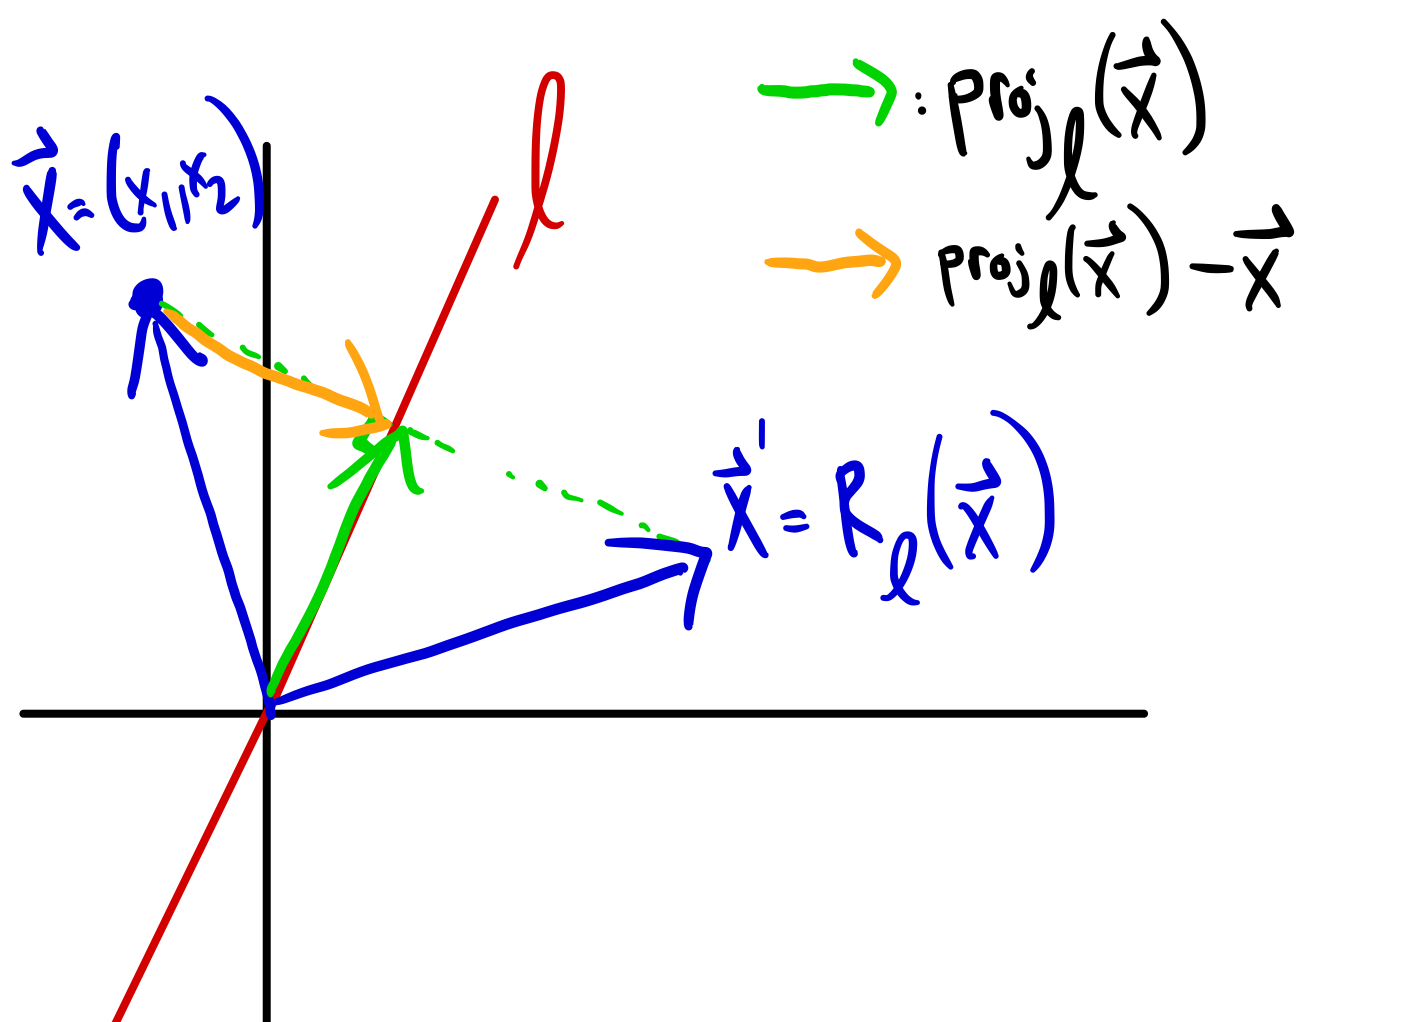
\includegraphics[width=3in]{Images/Reflection}
%\]
%\bpause 
%As the diagram illustrates, we have 
%\[
%R_\ell(\boldx)=\boldx+2(\proj{\boldx}{\ell}-\boldx)=2\proj{\boldx}{\ell}-\boldx=(2T_\ell-I_{\R^2})(\boldx),
%\]
%where $T_\ell$ is orthogonal projection onto $\ell$. 
%\end{frame}
%\begin{frame}{Reflection in $\R^2$}
%\[
%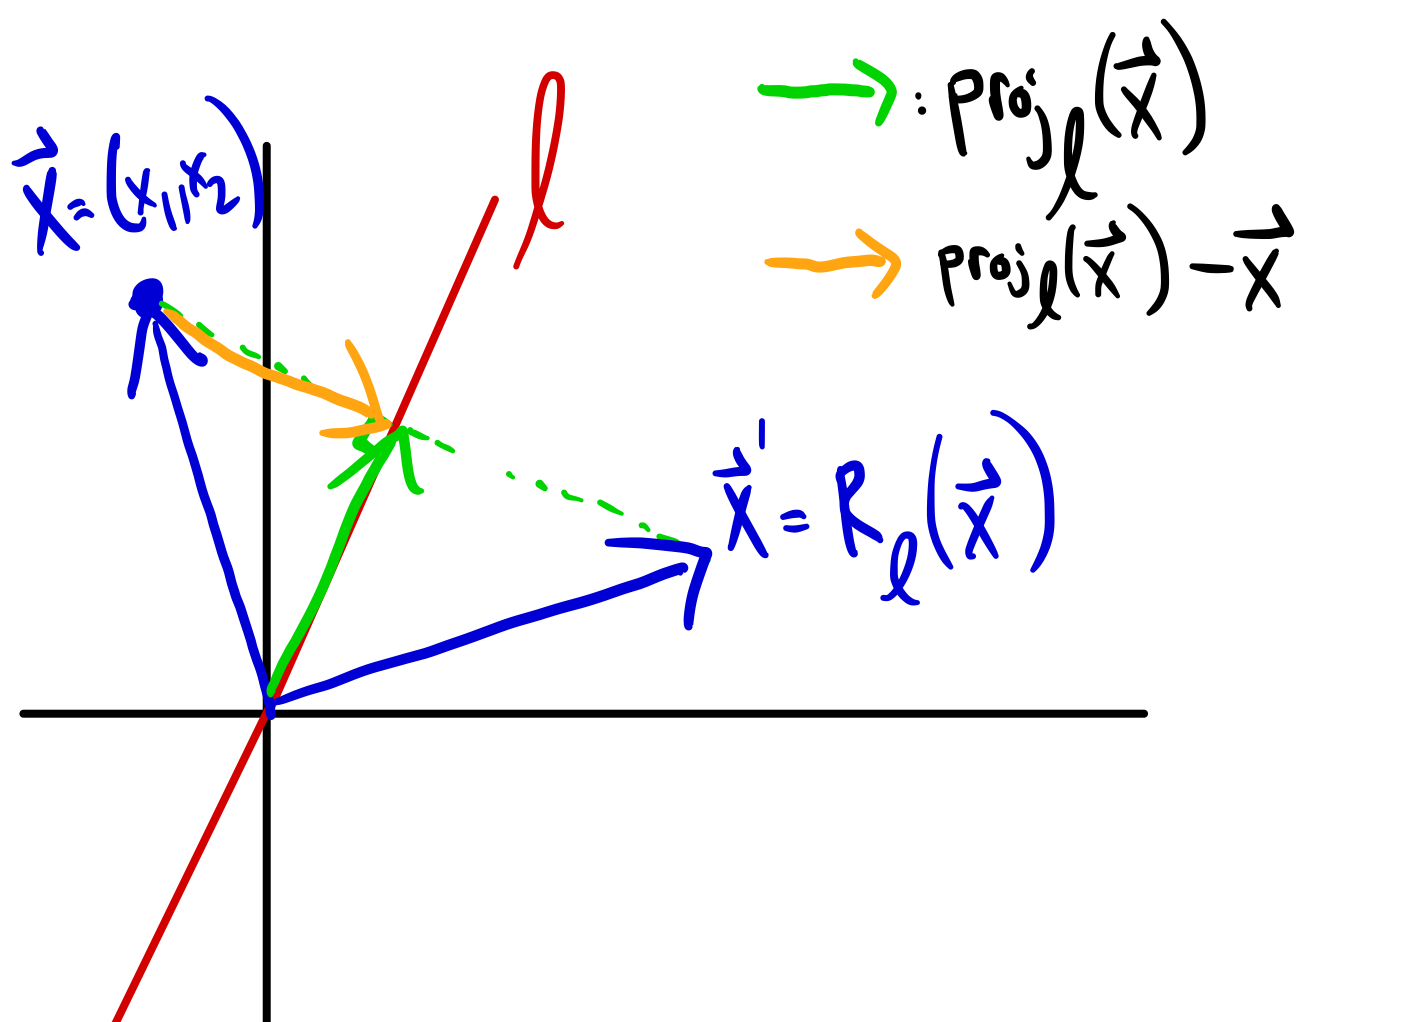
\includegraphics[width=.75in]{Images/Reflection}
%\]
%As the diagram illustrates, we have 
%\[
%R_\ell(\boldx)=\boldx+2(\proj{\boldx}{\ell}-\boldx)=2\proj{\boldx}{\ell}-\boldx=(2T_\ell-I_{\R^2})(\boldx),
%\]
%where $T_\ell$ is orthogonal projection onto $\ell$. 
%\bpause
%Write $\ell=\Span\{(y_1,y_2)\}$ for some vector $\boldy=(y_1,y_2)$. Then using our result about orthogonal projections, we have 
%\[
%R_{\ell}(x_1,x_2)=(2T_{\ell}-I_{\R^2})(x_1,x_2)=\left(\frac{2}{y_1^2+y_2^2}\begin{bmatrix}
%y_1^2&y_1y_2\\
%y_1y_2&y_2^2
%\end{bmatrix}-\begin{bmatrix}
%1&0\\
%0&1
%\end{bmatrix}\right) \begin{bmatrix}
%x_1\\ x_2
%\end{bmatrix}.
%\]
%\pause 
%This shows that $R_\ell=T_A$, where 
%\[
%A=\frac{2}{y_1^2+y_2^2}\begin{bmatrix}
%y_1^2&y_1y_2\\
%y_1y_2&y_2^2
%\end{bmatrix}-\begin{bmatrix}
%1&0\\
%0&1
%\end{bmatrix}=\frac{1}{y_1^2+y_2^2}\begin{bmatrix}
%y_1^2-y_2^2&2y_1y_2\\
%2y_1y_2&-y_1^2+y_2^2
%\end{bmatrix} .
%\]
%In particular, reflection through lines passing through the origin is linear!
%\bpause Note further, that if we let $\phi$ be the angle between $\boldy=(y_1,y_2)$ and $(1,0)$, then 
%\[
%A=\begin{bmatrix}\cos 2\phi&\sin 2\phi\\
%\sin 2\phi&-\cos 2 \phi
%\end{bmatrix}
%\]
%\end{frame} 
\begin{frame}{Exotic example: \alert{shift transformations}}
 Let $V=\R^\infty$, the vector space of all infinite sequences. 
 
 The {\bf left-shift transformation}, denoted $T_\ell$ is the function $T_\ell\colon \R^\infty\rightarrow\R^\infty$ defined as 
 \[
 T_\ell\left( (a_1,a_2,a_3,\dots)\right)=(a_2,a_3,\dots).
 \]
 
 The {\bf right-shift transformation}, denoted $T_r$ is the function $T_r\colon \R^\infty\rightarrow\R^\infty$ defined as 
 \[
 T_r\left( (a_1,a_2,a_3,\dots)\right)=(0,a_1,a_2,a_3,\dots).
 \]
 \pause
 In other words, $T_\ell$ takes an input sequence and returns as an output the sequence obtained by shifting all terms one to the left; $T_r$ takes an input sequence and returns as an output the sequence obtained by shifting all terms one to the right and setting the first term equal to 0. 
 \bpause
 \alert{Claim}: $T_\ell$ and $T_r$ are both linear transformations.
 \begin{proof}
 Exercise.
 \end{proof}
\end{frame}
\begin{frame}{Exotic example: \alert{differentiaton}}
Let $V=C^\infty(\R)$, the vector space of all infinitely differentiable functions on $\R$. 
\bspace
Define $T\colon C^\infty(\R)\rightarrow C^\infty(\R)$ by $T(f)=f'$. 
\bspace
In other words, $T$ takes as an input a function $f$, and returns as an output its derivative function $f'$. 
\bpause
\alert{Claim}: $T$ is a linear transformation. 
\pause \begin{proof}
We must show $T(cf+dg)=cT(f)+dT(g)$ for any scalars $c,d\in\R$ and any functions $f, g\in C^\infty(\R)$. 
\bpause
This follows easily from certain properties of the derivative: 
\begin{align*}
T(cf+dg)&=(cf+dg)' &\text{(def. of $T$)}\\
&=(cf)'+(dg)'&\text{(addition prop. of derivative)}\\
&=cf'+dg' &\text{(scalar prop. of derivative)}\\
&=cT(f)+dT(g) &\text{(def. of $T$)}
\end{align*}
\end{proof}
\end{frame}
%\begin{frame}{More examples}
%\footnotesize
%\bb
%\pause\ii Let $V=P_n$ and $W=P_{n+1}$, the function
%\begin{eqnarray*}
%T\colon P_n&\rightarrow& P_{n+1}\\
%p=p(x)\in P_{n}&\mapsto& T(p):=x\cdot p(x)
%\end{eqnarray*}
%is a linear transformation. 
%\pause\ii Let $V=M_{mn}$, $W=M_{nm}$. The function 
%\begin{eqnarray*}
%T\colon M_{mn}&\rightarrow& M_{nm}\\
%A\in M_{mn}&\mapsto&T(A):=A^T
%\end{eqnarray*}
%is a linear transformation. 
%\pause\ii Let $V=C^1(-\infty,\infty)$, $W=C(-\infty,\infty)$. The function 
%\begin{eqnarray*}
%T\colon C^1(-\infty,\infty)&\rightarrow& C(-\infty,\infty)\\
%f\in C^1(-\infty,\infty)&\mapsto& T(f):=f'
%\end{eqnarray*}
%is a linear transformation. 
%\bpause
%More generally, taking $f$ to its $n$-th derivative $f^{(n)}$ is a linear transformation for any $n$ thanks to the sum and scalar multiplication rules of differentiation! This property is very important in the theory of linear differential equations. 
%\ee
%\end{frame}
%\begin{frame}{Null space and range}
%\begin{definition}
%Let $V$ and $W$ be vector spaces, and $T\colon V\rightarrow W$ a linear transformation. We define
%\begin{eqnarray*}
%\NS(T)&:=&\{\boldv\in V\colon T(\boldv)=\boldzero_W\}\subseteq V\\
%\range(T)&:=&\{\boldw\in W\colon \boldw=T(\boldv)\text{ for some } \boldv\in V\}\subseteq W
%\end{eqnarray*}
%\end{definition}
%\pause
%\alert{Comments}.
%\bb
%\ii In the literature  $\NS(T)$ is also called the {\bf kernel} of $T$, denoted $\ker(T)$. I'll just stick to $\NS(T)$. 
%\pause\ii Both $\NS(T)$ and $\range(T)$ are indeed \alert{subspaces}. Note that they live in different spaces: $\NS(T)\subseteq V$ and $\range(T)\subseteq W$.  
%\pause\ii We define $\nullity(T)=\dim(\NS(T))$ and $\rank(T)=\dim(\range(T))$.
%\pause
%\ii When we are in the special case where $T_A\colon \R^n\rightarrow \R^m$ for some matrix $A\in M_{mn}$, it is easy to see that $\NS(T_A)=\NS(A)$ and $\range(T_A)=\CS(A)$.     
%\ee
%\end{frame}
%\begin{frame}{Proof that $\range(T)$ is a subspace}
%\footnotesize
%We continue to assume $T\colon V\rightarrow W$ is a linear transformation. Let's show $\range(T)=\{\boldw\in W\colon \boldw=T(\boldv)\text{ for some } \boldv\in V\}$ is a subspace. 
%\bb[(i)]
%\pause\ii We must show $\boldzero_W\in \range(T)$. But $\boldzero_W=T(\boldzero_V)$. Thus there is a $\boldv\in V$ with $T(\boldv)=\boldzero_W$, which proves that $\boldzero_W\in\range(T)$. 
%\pause\ii Suppose $\boldw_1,\boldw_2\in \range(T)$. This means there are $\boldv_1, \boldv_2\in V$ such that $T(\boldv_i)=\boldw_i$ for $i=1,2$. We must show $\boldw=\boldw_1+\boldw_2\in\range(T)$.  
%\bpause 
%Set $\boldv=\boldv_1+\boldv_2$. Then
%\begin{eqnarray*}
%T(\boldv)&=&T(\boldv_1+\boldv_2)\\
%&=&T(\boldv_1)+T(\boldv_2) \ \text{ (since $T$ is a linear transformation)}\\
%&=&\boldw_1+\boldw_2=\boldw.
%\end{eqnarray*} 
%Since we have provided a $\boldv$ with $T(\boldv)=\boldw_1+\boldw_2$, we see that $\boldw_1+\boldw_2\in\range(T)$. 
%\pause\ii Suppose $\boldw\in\range(T)$. Then there is a $\boldv\in V$ with $T(\boldv)=\boldw$. Then $T(k\boldv)=kT(\boldv)=k\boldw$, showing $k\boldw\in\range(T)$.  
%\ee
%\end{frame}
%\begin{frame}{Example: orthogonal projection}
% Let $(V, \angvec{\ , })$ be an inner product space, and let $W\subseteq V$ be a \alert{finite-dimensional} subspace. We showed in a homework exercise that the orthogonal projection map: 
% \begin{align*}
% \text{proj}_W\colon V&\rightarrow V\\
% \boldv&\mapsto \proj{\boldv}{W}
% \end{align*} 
% satisfies $\proj{c_1\boldv_1+c_2\boldv_2}{W}=c_1\proj{\boldv_1}{W}+c_2\proj{\boldv_2}{W}$. 
% \bpause 
% Thus orthogonal projection defines a linear transformation from $V$ to $V$. 
%\bpause
%\alert{Null space}. We showed in homework that $\proj{\boldv}{W}=\boldzero$ if and only if $\boldv\in W^\perp$. Thus 
%\[
%\NS(\text{proj}_W)=W^\perp.
%\]
%\bpause
%\alert{Range}.  It is easy to see that $\range(\text{proj}_W)=W$. Indeed, we have $\proj{\boldv}{W}\subseteq W$ by definition. Going the other way, given any $\boldw\in W$, we have $\proj{\boldw}{W}=\boldw$. Thus $W\subseteq \range(\text{proj}_W)$. 
%\end{frame} 
%
%\begin{frame}
%\begin{theorem}[Rank-nullity theorem]
%Let $V$ and $W$ be spaces, $T\colon V\rightarrow W$ a linear transformation. Suppose further that $V$ is \alert{finite-dimensional}. Then 
%\[
%\dim(V)=\dim(\NS(T))+\dim(\range(T).
%\]
%\end{theorem}
%\pause
%\begin{proof}
%Let $\dim V=n$. Since $V$ is finite-dimensional and $\NS(T)\subseteq V$, it follows that $\NS(T)$ is finite-dimensional. 
%\\
%\pause Let $S=\{\boldv_1,\boldv_2,\dots, \boldv_r\}$ be a basis of $\NS(T)$; \alert{extend} this basis to a full basis $\{\boldv_1,\boldv_2,\dots, \boldv_r, \boldu_{1},\dots \boldu_{n-r}\}$ of $V$. 
%\\
%\pause Claim: $S'=\{T(\boldu_{1}),\dots, T(\boldu_{n-r})\}$ is a basis of $\range(T)$. If this is true we are done, since we have $\dim(\NS(T))=\#S=r$ and $\dim(\range(T))=\#S'=n-r$,  and thus 
%\[
%\dim(V)=n=r+(n-r)=\dim(\NS(T))+\dim(\range(T).
%\]
%\pause Now ask your professor to prove the claim. 
%\end{proof}
%\end{frame}
%\begin{frame}{Linear transformations and bases}
%\begin{theorem}
%Let $S=\{\boldv_1,\dots,\boldv_n\}$ be a basis for $V$, and let $W$ be any space. 
%\bb[(a)]
%\ii Given any choice of $n$ elements $\boldw_1,\boldw_2,\dots, \boldw_n\in W$ there is a \alert{unique} linear transformation $T\colon V\rightarrow W$ such that $T(\boldv_i)=\boldw_i$. 
%\ii Given linear transformations $T_1,T_2\colon V\rightarrow W$, $T_1=T_2$ if and only if $T_1(\boldv_i)=T_2(\boldv_i)$ for $1\leq i\leq n$.  
%\ee
%\end{theorem}
%\pause
%This is an extremely useful theorem as it allows us, given a basis $S$ of $V$, to 
%\bb[(i)]
%\ii easily define linear transformations simply by declaring where $\boldv_i$ gets sent for each $i$, and 
%\pause \ii easily check whether two linear transformations are equal simply by checking that they agree on the basis elements $\boldv_i$. 
%\ee
%\end{frame}
%\begin{frame}{Transformations of $\R^n$}
%An important corollary of this theorem is the fact that \alert{every} linear transformation $T\colon\R^n\rightarrow\R^m$ between is given by a matrix: that is, $T=T_A$ for some $m\times n$ matrix $A$. 
%\bspace 
%Indeed, given such a $T$, let $A$ be the matrix whose $j$-th column is $\boldc_j=T(\bolde_j)$, where $\bolde_j$ is the $j$-th element of the standard basis of $\R^n$. I claim $T=T_A$. 
%\pause
%\begin{proof}
%According to the theorem, I only need to show that $T$ and $T_A$ agree on any basis of $\R^n$. Let's take the standard basis $B=\{\bolde_1,\dots,\bolde_n\}$. 
%
%\pause Then 
%\begin{align*}
%T_A(\bolde_j)&=A\bolde_j &\text{(def. of $T_A$) }\\
%&=\boldc_j &\text{(column expansion)}\\
%&=T(\bolde_j) &\text{(def. of $A$)}
%\end{align*}
%We've shown that $T_A(\bolde_j)=T(\bolde_j)$ for all $\bolde_j\in B$. The theorem implies $T=T_A$. 
%\end{proof}
%\end{frame}
%\begin{frame}{Example: rotations}
%Fix an angle $\theta$ and consider the map $T_\theta\colon\R^2\rightarrow\R^2$ that takes a vector $\boldx$ and maps it to the vector $\boldy=T_\theta(\boldx)$ you get by rotating $\boldx$ by $\theta$, taking counterclockwise to be the positive direction. We call this map a \alert{rotation} by $\theta$. 
%\bpause
%Take for granted for the time being that $T_\theta$ is in fact a linear transformation (not totally obvious). Find the matrix $A_\theta$ that represents this linear transformation. 
%\begin{bsolution}
%According to the previous slide we have 
%\[
%A_\theta=\begin{bmatrix}\vert &\vert\\ T_\theta(\bolde_1)&T_\theta(\bolde_2)\\ \vert &\vert \end{bmatrix},
%\]
%where $\bolde_1=\begin{bmatrix}
%1\\0
%\end{bmatrix} $ and $ \bolde_2=\begin{bmatrix}
%0\\1
%\end{bmatrix}$, as usual.  \pause A simple drawing on the unit circle tells us what happens to these vectors when we rotate them by $\theta$. We get:
%\[
%T_\theta(\bolde_1)=\begin{bmatrix}
%\cos(\theta)\\ \sin(\theta)
%\end{bmatrix}, T_\theta(\bolde_2)=\begin{bmatrix}
%-\sin(\theta)\\ \cos(\theta)
%\end{bmatrix}
%\]
%Thus 
%\[
%A_\theta=\begin{bmatrix}
%\cos(\theta)&-\sin(\theta)\\ \sin(\theta) &\cos(\theta)
%\end{bmatrix}
%\]
%We call this a \alert{rotation matrix}.  
%\end{bsolution} 
%\end{frame}
%\begin{frame}{Projection onto a line in $\R^n$, $n=2,3$}
%Let $V=\R^n$ for $n=2$ or $n=3$, and let $\ell\subseteq V$ be a line passing through the origin. Define $T_\ell$ to be the transformation that takes a vector $\boldx$ and returns its \alert{orthogonal projection} $\proj{\boldx}{\ell}$ onto $\ell$: i.e., we define $T_\ell(\boldx)=\proj{\boldx}{\ell}$. 
%\bpause
%We have $\ell=\Span\{\boldy\}$ for some vector $\boldy\in \R^n$. In multivariable calculus we derive a dot product formula orthogonal projection: namely, $\proj{\boldx}{\ell}=(\frac{\boldx\cdot\boldy}{\boldy\cdot\boldy})\boldy$. We can use this formula to identify $T_\ell=T_A$ for a matrix $A\in M_{nn}$. We treat $n=2, 3$ separately.  
%\bpause
%{\color{blue} Case $n=2$}. Let $\boldy=(y_1,y_2)$. For $(x_1, x_2)$ we have 
%\[
%\proj{(x_1,x_2)}{\ell}=\frac{y_1x_1+y_2x_2}{y_1^2+y_2^2}(y_1,y_2)=\frac{1}{y_1^2+y_2^2}\begin{bmatrix}
%y_1^2&y_1y_2\\
%y_1y_2&y_2^2
%\end{bmatrix} \begin{bmatrix}
%x_1\\ x_2
%\end{bmatrix} 
%\]
%\bpause
%{\color{blue} Case $n=3$}. Let $\boldy=(y_1,y_2,y_3)$. For $(x_1, x_2,x_3)$ we have 
%\[
%\proj{(x_1,x_2,x_3)}{\ell}=\frac{y_1x_1+y_2x_2+y_3x_3}{y_1^2+y_2^2+y_3^2}(y_1,y_2,y_3)=\frac{1}{y_1^2+y_2^2+y_3^2}\begin{bmatrix}
%y_1^2&y_1y_2&y_1y_3\\
%y_1y_2&y_2^2&y_2y_3\\
%y_1y_3&y_2y_3&y_3^2
%\end{bmatrix} \begin{bmatrix}
%x_1\\ x_2\\x_3
%\end{bmatrix} 
%\]
%\pause 
%Thus $T_\ell=T_A$ where $A=\frac{1}{y_1^2+y_2^2}\begin{bmatrix}
%y_1^2&y_1y_2\\
%y_1y_2&y_2^2
%\end{bmatrix}$ in the $n=2$ case, and $A=\frac{1}{y_1^2+y_2^2+y_3^2}\begin{bmatrix}
%y_1^2&y_1y_2&y_1y_3\\
%y_1y_2&y_2^2&y_2y_3\\
%y_1y_3&y_2y_3&y_3^2
%\end{bmatrix}$ in the $n=3$ case.
%\end{frame} 
%\begin{frame}{Reflection in $\R^2$}
%Let $V=\R^2$. Given an arbitrary line $\ell$ passing through the origin, let $R_\ell$ be the transformation that maps a vector $\boldx$ to its reflection $\boldx'=R_\ell(\boldx)$ across $\ell$. 
%\[
%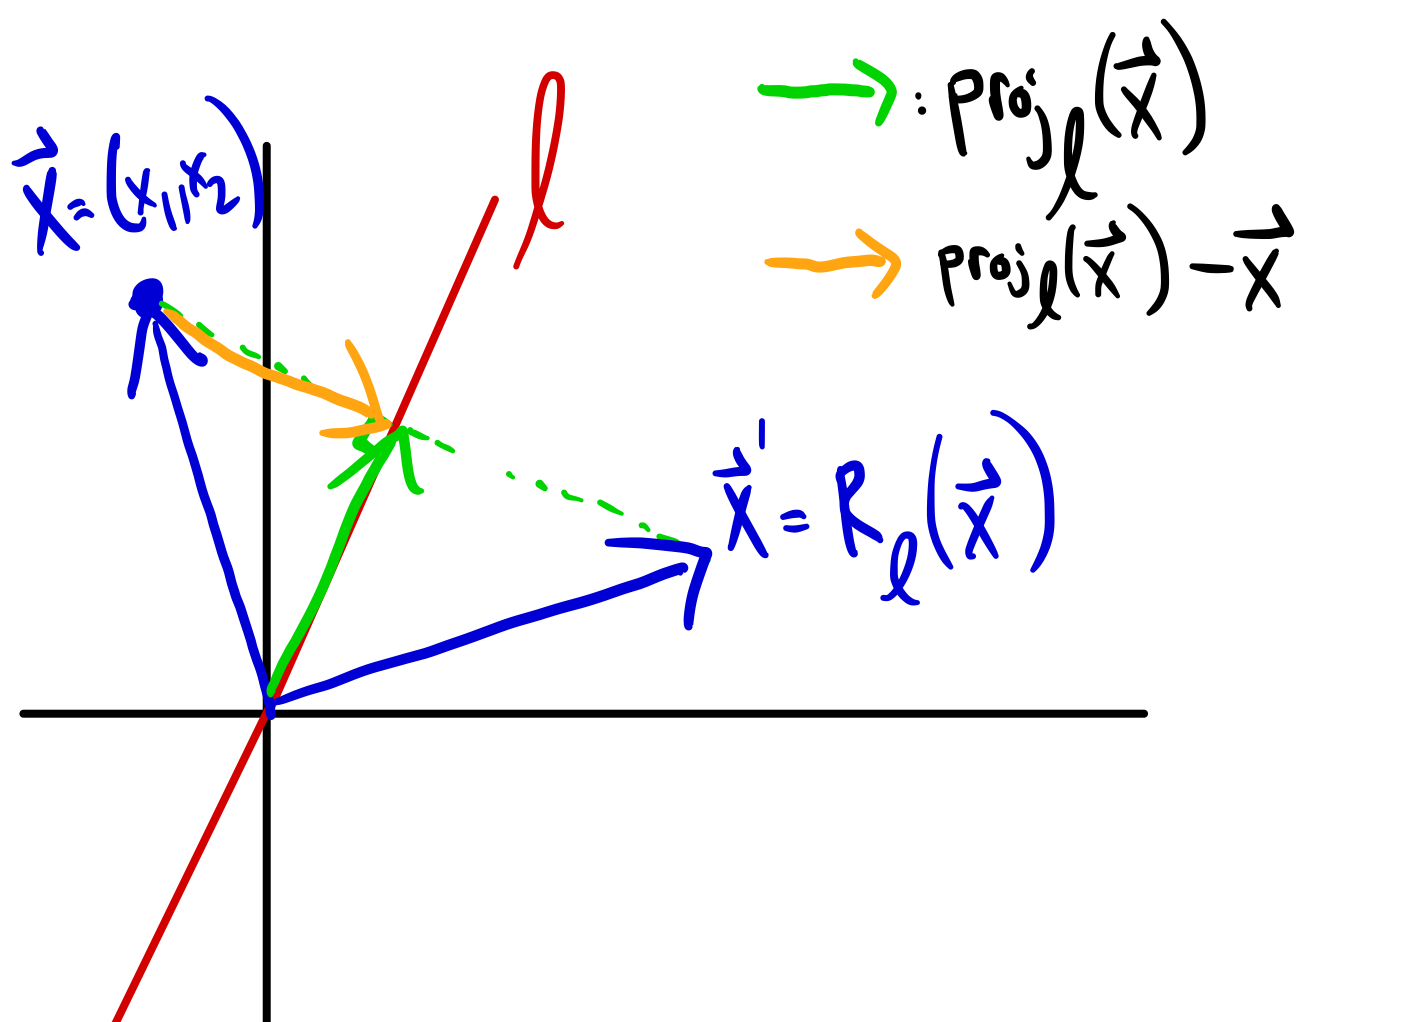
\includegraphics[width=3in]{Images/Reflection}
%\]
%\bpause 
%As the diagram illustrates, we have 
%\[
%R_\ell(\boldx)=\boldx+2(\proj{\boldx}{\ell}-\boldx)=2\proj{\boldx}{\ell}-\boldx=(2T_\ell-I_{\R^2})(\boldx),
%\]
%where $T_\ell$ is orthogonal projection onto $\ell$. 
%\end{frame}
%\begin{frame}{Reflection in $\R^2$}
%\[
%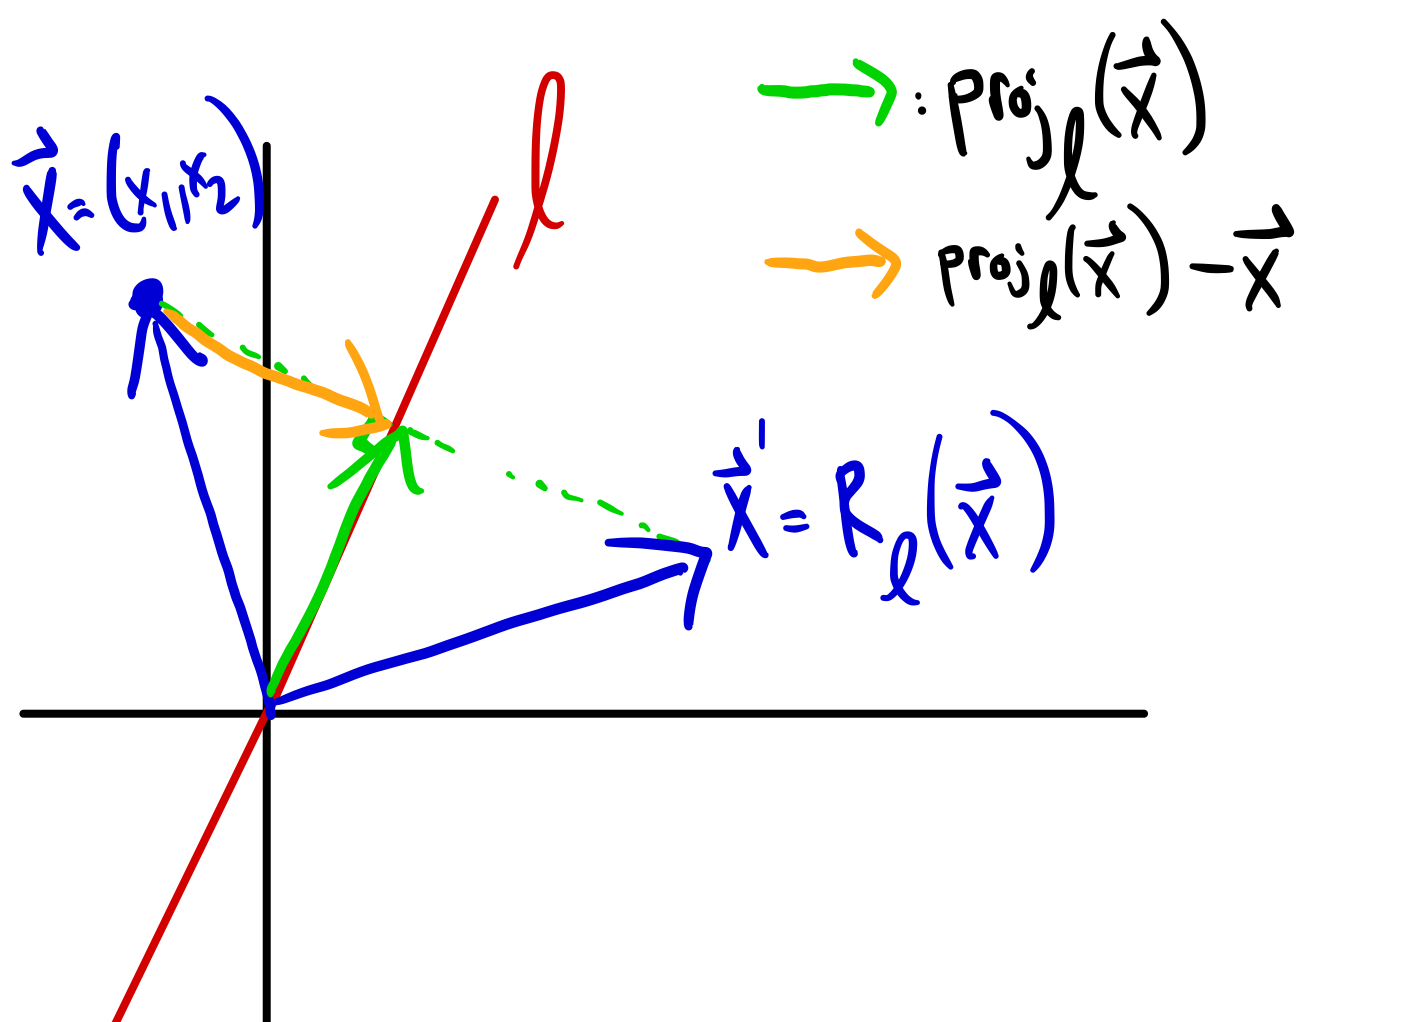
\includegraphics[width=.75in]{Images/Reflection}
%\]
%As the diagram illustrates, we have 
%\[
%R_\ell(\boldx)=\boldx+2(\proj{\boldx}{\ell}-\boldx)=2\proj{\boldx}{\ell}-\boldx=(2T_\ell-I_{\R^2})(\boldx),
%\]
%where $T_\ell$ is orthogonal projection onto $\ell$. 
%\bpause
%Write $\ell=\Span\{(y_1,y_2)\}$ for some vector $\boldy=(y_1,y_2)$. Then using our result about orthogonal projections, we have 
%\[
%R_{\ell}(x_1,x_2)=(2T_{\ell}-I_{\R^2})(x_1,x_2)=\left(\frac{2}{y_1^2+y_2^2}\begin{bmatrix}
%y_1^2&y_1y_2\\
%y_1y_2&y_2^2
%\end{bmatrix}-\begin{bmatrix}
%1&0\\
%0&1
%\end{bmatrix}\right) \begin{bmatrix}
%x_1\\ x_2
%\end{bmatrix}.
%\]
%\pause 
%This shows that $R_\ell=T_A$, where 
%\[
%A=\frac{2}{y_1^2+y_2^2}\begin{bmatrix}
%y_1^2&y_1y_2\\
%y_1y_2&y_2^2
%\end{bmatrix}-\begin{bmatrix}
%1&0\\
%0&1
%\end{bmatrix}=\frac{1}{y_1^2+y_2^2}\begin{bmatrix}
%y_1^2-y_2^2&2y_1y_2\\
%2y_1y_2&-y_1^2+y_2^2
%\end{bmatrix} .
%\]
%In particular, reflection through lines passing through the origin is linear!
%\bpause Note further, that if we let $\phi$ be the angle between $\boldy=(y_1,y_2)$ and $(1,0)$, then 
%\[
%A=\begin{bmatrix}\cos 2\phi&\sin 2\phi\\
%\sin 2\phi&-\cos 2 \phi
%\end{bmatrix}
%\]
%\end{frame} 
%\begin{frame}{Example: orthogonal projection in $\R^2$}
% Consider $\R^3$ with the dot product, and let $W$ be the plane orthogonal to the vector $\boldn=(a,b,c)$. For $\boldx\in\R^3$, define $T(\boldx)$ to be the orthogonal projection of 
% 
%  \bpause 
% We derived a formula for $A$ in terms of $a,b,c$ earlier. We do so again, this time column by column: 
% \pause
% \begin{align*}
% \proj{\bolde_1}{W}&=\bolde_1-\proj{\bolde_1}{W^\perp}=\bolde_1-\frac{\bolde_1\cdot \boldn}{\boldn\cdot\boldn}\boldn=\frac{1}{a^2+b^2+c^2}\colvec{b^2+c^2\\ -ab\\ -ac}\\
% \proj{\bolde_2}{W}&=\bolde_2-\proj{\bolde_2}{W^\perp}=\bolde_2-\frac{\bolde_2\cdot \boldn}{\boldn\cdot\boldn}\boldn=\frac{1}{a^2+b^2+c^2}\colvec{-ab\\ a^2+c^2\\ -bc}\\
% \proj{\bolde_3}{W}&=\bolde_3-\proj{\bolde_3}{W^\perp}=\bolde_3-\frac{\bolde_3\cdot \boldn}{\boldn\cdot\boldn}\boldn=\frac{1}{a^2+b^2+c^2}\colvec{-ac\\ -bc\\ a^2+b^2}
% \end{align*} 
% \pause Thus $\text{proj}_W=T_A$, where $A=\frac{1}{a^2+b^2+c^2}\begin{bmatrix}
%  b^2+c^2& -ab&-ac\\
%  -ab&a^2+c^2&-bc\\
%  -ac&-bc&a^2+b^2
% \end{bmatrix} 
% $
%\end{frame} 
%\begin{frame}{Example: orthogonal projection in $\R^3$}
% Consider $\R^3$ with the dot product, and let $W$ be the plane orthogonal to the vector $\boldn=(a,b,c)$. Since $\text{proj}_W\colon\R^3\rightarrow \R^3$ is a linear transformation of $\R^3$, we must have $\text{proj}_W=T_A$ for some $A\in M_{33}$. 
% \bpause 
% We derived a formula for $A$ in terms of $a,b,c$ earlier. We do so again, this time column by column: 
% \pause
% \begin{align*}
% \proj{\bolde_1}{W}&=\bolde_1-\proj{\bolde_1}{W^\perp}=\bolde_1-\frac{\bolde_1\cdot \boldn}{\boldn\cdot\boldn}\boldn=\frac{1}{a^2+b^2+c^2}\colvec{b^2+c^2\\ -ab\\ -ac}\\
% \proj{\bolde_2}{W}&=\bolde_2-\proj{\bolde_2}{W^\perp}=\bolde_2-\frac{\bolde_2\cdot \boldn}{\boldn\cdot\boldn}\boldn=\frac{1}{a^2+b^2+c^2}\colvec{-ab\\ a^2+c^2\\ -bc}\\
% \proj{\bolde_3}{W}&=\bolde_3-\proj{\bolde_3}{W^\perp}=\bolde_3-\frac{\bolde_3\cdot \boldn}{\boldn\cdot\boldn}\boldn=\frac{1}{a^2+b^2+c^2}\colvec{-ac\\ -bc\\ a^2+b^2}
% \end{align*} 
% \pause Thus $\text{proj}_W=T_A$, where $A=\frac{1}{a^2+b^2+c^2}\begin{bmatrix}
%  b^2+c^2& -ab&-ac\\
%  -ab&a^2+c^2&-bc\\
%  -ac&-bc&a^2+b^2
% \end{bmatrix} 
% $
%\end{frame} 
